%!TEX root = ../dokumentation.tex

\chapter{Materialien und Methoden} \label{ch:materialsAndMethods}

Die deutsche Politik in der 19. Legislaturperiode wird durch die Bundestagswahl 2017 geprägt, die als Ausgangspunkt für die politischen Entwicklungen in diesem Zeitraum diente. Die Heterogenität der Parteilandschaft und besondere Ereignisse während dieser Legislaturperiode trugen zur Vielfalt der politischen Strömungen und Dynamiken bei. Durch die politischen Akteure werden verschiedene Themenschwerpunkte gesetzt, um politische Agenden zu gestalten und Herausforderungen anzugehen.

Im Bereich der Textanalyse werden verschiedene Repräsentationsformen von Text wie N-Grams, \ac{BoW}, \ac{TF-IDF}, \ac{GloVe}, \ac{CNN}-Embedding-Schicht, \ft und \ac{BERT} untersucht. Jede Methode weist ihre eigenen Vor- und Nachteile bei der Verarbeitung und Darstellung von Textdaten auf. Zusätzlich wird ein Modell zur Sentimentanalyse für die deutsche Sprache vorgestellt. Dieses soll dazu genutzt werden, um die Datensätze in \autoref{ch:crispDm_1} zu analysieren.

\section{Deutsche Politik in der 19. Legislaturperiode}

Dieser Abschnitt bietet einen Überblick über die politische Situation während der \num{19}. Wahlperiode des Deutschen Bundestages. Die politischen Themen und Aussagen werden in den zu untersuchenden Texten widergespiegelt. In \autoref{subsec:btw17} wird der Ausgang und die Folgen der Bundestagswahl \num{2017} beleuchtet und im Anschluss daran werden in \autoref{subsec:heterogenitätParteien} die Parteienlandschaft sowie parteiinterne Unterschiede und Flügel näher betrachtet. In \autoref{subsec:besondereEreignisse} werden besondere Ereignisse im Untersuchungszeitraum aufgelistet und in \autoref{subsec:themenschwerpunkte} diejenigen Themen erläutert, die während der Zeit den politischen Diskurs am stärksten geprägt haben.

\subsection{Bundestagswahl \num{2017}} \label{subsec:btw17}

Die Bundestagswahl \num{2017} wurde am \num{24}. September \num{2017} abgehalten. \autoref{fig:ergebnisBtw17} zeigt die Aufteilung der Zweitstimmen nach Partei.

\begin{figure}[H]
  \centering
  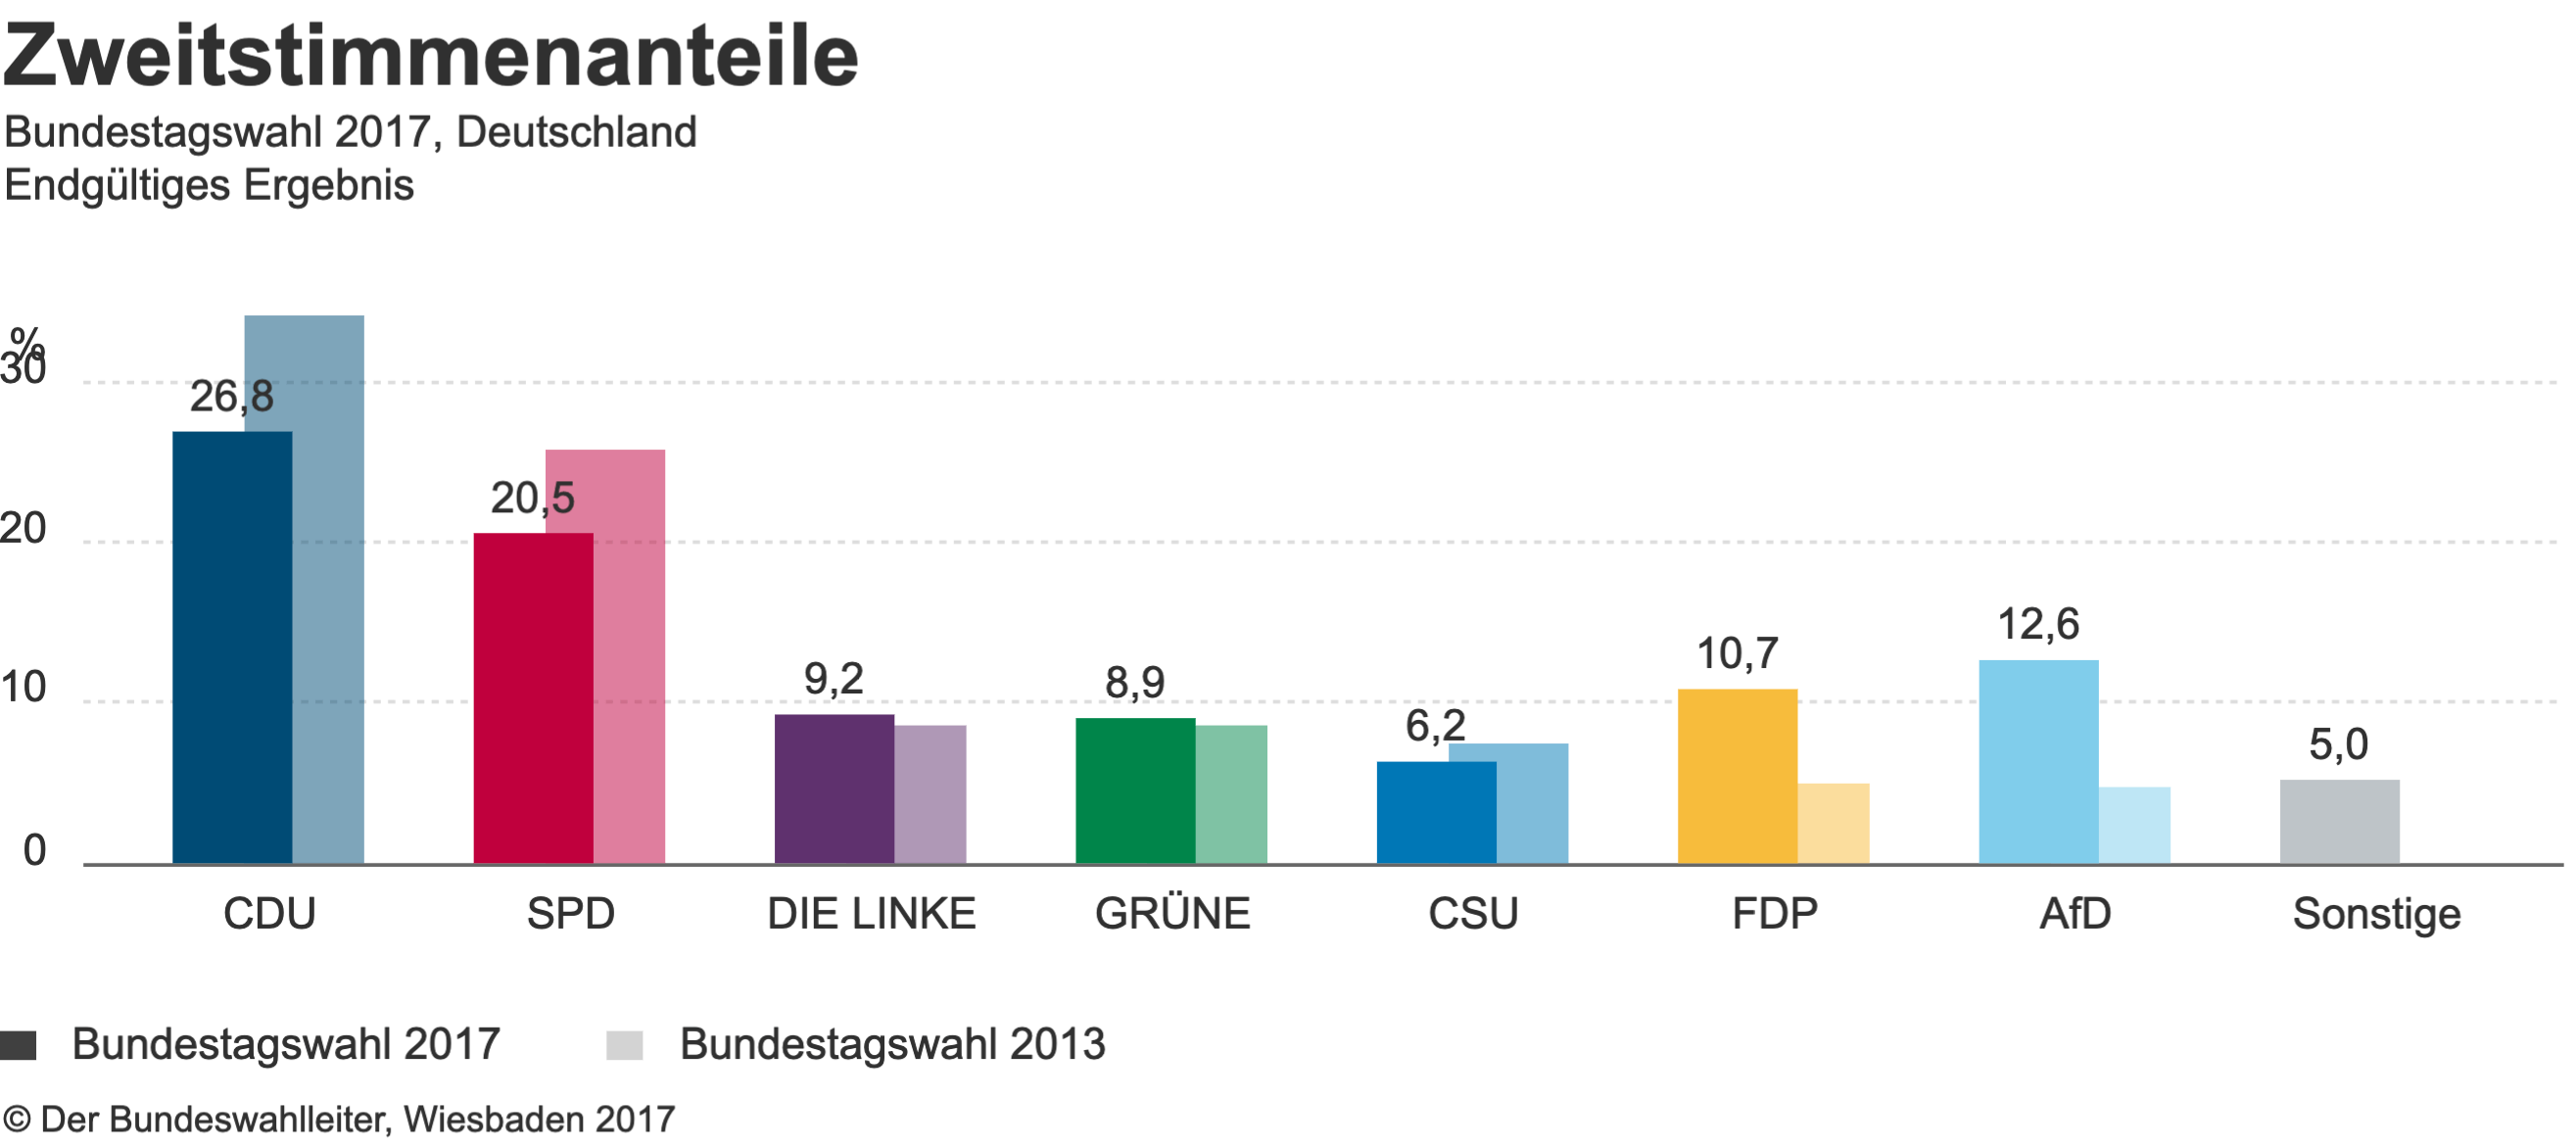
\includegraphics[width=0.9\textwidth]{data/images/ergebnisBtw17.png}
  \caption{Ergebnis der Bundestagswahl \num{2017} \autocite{noauthor_bundestagswahl_nodate}} \label{fig:ergebnisBtw17}
\end{figure}

Die \ac{CDU} hat zwar einen starken Verlust im Vergleich zur vorherigen Wahl erlitten, konnte sich aber dennoch mit \SI{26.8}{\percent} der Stimmen als stärkste Kraft durchsetzen. Gemeinsam haben die \ac{CDU} und \acs{CSU} insgesamt \SI{32.9}{\percent} erreicht. Die \ac{SPD}, die ebenfalls im Vergleich zur Bundestagswahl \num{2013} an Stimmen verloren hat, kam auf \SI{20.5}{\percent}. Mit minimalen Steigerungen haben die Linke \SI{9.2}{\percent} und die Grünen \SI{8.9}{\percent} erreicht. Sowohl die \ac{FDP} mit \SI{10.7}{\percent} als auch die \ac{AfD} mit \SI{12.6}{\percent} konnten ihre Anteile deutlich steigern. Während die \ac{AfD} durch dieses Ergebnis zum ersten Mal in den Bundestag einziehen konnte, war es der \ac{FDP} nach dem Ausscheiden \num{2013} möglich, erneut in den Bundestag einzuziehen. Die übrigen Parteien erreichten kumuliert \SI{5}{\percent} der Stimmen.

Laut \textcite{schmid_deutscher_2021} waren nach der Bundestagswahl \num{2017} zum ersten Mal sieben Parteien und sechs Fraktionen im Bundestag vertreten, was als Zeichen für die weiter abnehmende Bindungskraft der Volksparteien \ac{CDU}, \ac{CSU} und \ac{SPD} gesehen werden kann. Besonders hervorzuheben sind dabei die starken Verluste von Union und \ac{SPD}. Die \ac{SPD} hat mit dieser Bundestagswahl ihr schlechtestes Ergebnis seit \num{1949} verzeichnet.

Nach der Wahl wurden Sondierungsverhandlungen für eine mögliche \enquote{Jamaika-Koalition} zwischen Union, \ac{FDP} und Grünen begonnen. Nachdem diese seitens der \ac{FDP} abgebrochen worden waren, bildete sich eine Große Koalition aus Union und \ac{SPD}. Damit wurde die längste Regierungsbildung in der Geschichte Deutschlands verzeichnet \parencite{schmid_deutscher_2021}.

\subsection{Heterogenität der Parteienlandschaft} \label{subsec:heterogenitätParteien}

Laut \textcite{niedermayer_entwicklung_2020} ist im deutschen Parteiensystem ein Wandel erkennbar, der von den traditionellen zwei Volksparteien (\ac{CDU} und \ac{SPD}) hin zu \enquote{einem pluralistischen System an der Grenze zum hochfragmentierten System} führt. Hierbei ist besonders bei den Volksparteien ein schrittweiser Verlust der Zustimmung festzustellen, während sich die Grünen als zweitstärkste Kraft etablieren konnten. Auch die \ac{AfD} hat sich fest verankert. Bei der \ac{FDP} und der Linken ist wenig Dynamik zu bemerken.

\textcite{engler_wettbewerb_2022} betonen, dass die Oppositionsparteien bei vielen Themen divergente Meinungen sowohl gegenüber der Regierung als auch untereinander vertreten. Während die Grünen und die Linke für konsequentere Klimamaßnahmen plädieren, positioniert sich die \ac{AfD} entgegengesetzt. In der Debatte um Corona-Maßnahmen ergibt sich ein ähnliches Bild, in dem auch die \ac{FDP} Kritik an einigen Maßnahmen geäußert hat.

Die politischen Parteien in Deutschland können grundsätzlich in zwei Lager eingeteilt werden: Ein \enquote{links-liberales}, bestehend aus \ac{SPD}, Grünen und Linken, sowie ein \enquote{rechts-konservatives} oder \enquote{bürgerliches}, bestehend aus der Union und \ac{AfD} \autocite{thomeczek_politische_2019}. Der \ac{FDP} wird eine Sonderrolle als gesellschaftspolitisch liberale, aber wirtschaftspolitisch rechte Partei zugeschrieben. Zudem beobachten \textcite{thomeczek_politische_2019}, dass die Parteien eine unterschiedliche interne Kohärenz aufweisen. Die beiden Volksparteien, \ac{SPD} und \ac{CDU}, zeigen dabei durchschnittlich geringere Agreement-Index-Werte -- ein Maßstab, der misst, wie stark die Positionen der Mitglieder übereinstimmen -- als die anderen Parteien.

Die Verteilung der Positionen innerhalb einer Partei betrachtet auch \textcite{saltzer_bundestagswahl_2022}. \autoref{fig:positionierungAusgewaehlterKanidaten} zeigt die Verortung von Kandidaten für die Bundestagswahl \num{2021} nach Partei. Die x-Achse stellt dabei die Position in der politischen Links-Rechts-Skala und die y-Achse die Zustimmung zu Regierung beziehungsweise Opposition dar.

\begin{figure}[H]
  \centering
  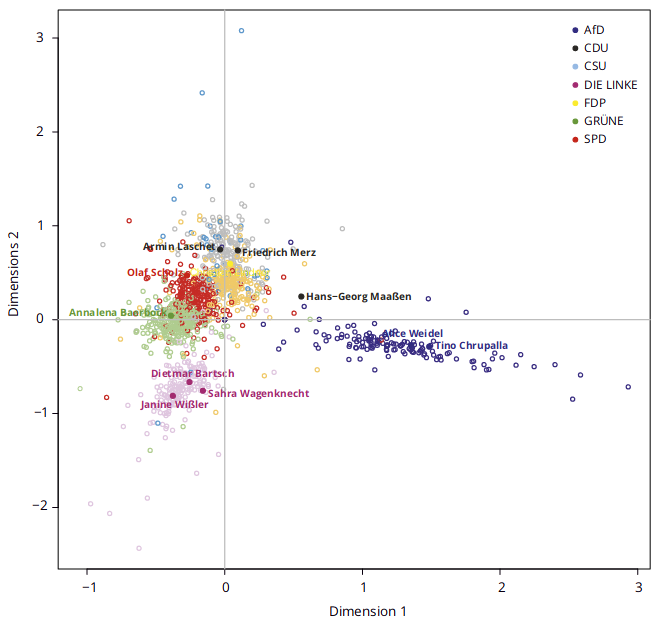
\includegraphics[width=0.5\textwidth]{data/images/positionierung_ausgewaehlter_kandidaten.png}
  \caption[Positionierung ausgewählter Kandidaten \autocite{saltzer_bundestagswahl_2022}]{Positionierung ausgewählter Kandidaten innerhalb eines zweidimensionalen politischen Raums \autocite{saltzer_bundestagswahl_2022}} \label{fig:positionierungAusgewaehlterKanidaten}
\end{figure}

Aus der Grafik geht hervor, dass sich insbesondere die Parteien an den Rändern des politischen Spektrums -- die Linke und die \ac{AfD} -- visuell von den übrigen Parteien abgrenzen. Die restlichen Parteien verteilen sich um den Ursprung des Koordinatensystems und überschneiden sich dabei auch.

Die Kandidaten der Union und der \ac{FDP} befinden sich im Schnitt in der Mitte der Links-Rechts-Skala. Dabei ist die Regierungs-Zustimmung der Union höher. Im Vergleich zur \ac{FDP} ist die \ac{SPD} weiter links positioniert. Die Kandidaten der Grünen sind noch weiter links verortet und neutral auf der y-Achse. Die Linke ist ähnlich weit links positioniert wie die Grünen, neigt aber deutlich stärker zur Opposition. Die \ac{AfD} ist die einzige Partei, die in der gegebenen Darstellung rechts der Mitte verortet ist und dabei eher der Opposition zuneigt.

Auffällig ist, dass die Verteilung der \ac{AfD}-Kandidaten auf der Links-Rechts-Skala deutlich stärker streut im Vergleich zu den anderen Parteien. Eine mögliche Begründung dafür ist der Protest gegen die etablierten Parteien. Daraus ergibt sich eine niedrigere interne Übereinstimmung bei politischen Themen und eine größere Streuung der Meinungen.

\subsection{Besondere Ereignisse im Untersuchungszeitraum} \label{subsec:besondereEreignisse}

\textcite{schmid_deutscher_2021} weist auf wichtige öffentlichkeitswirksame Ereignisse während der \num{19}. Wahlperiode des deutschen Bundestages hin. Darunter fällt zunächst die Corona-Pandemie, deren Auswirkungen und der Umgang mit diesen nach den ersten Ansteckungsfällen Anfang 2020 zu zentralen Themen in Politik und Gesellschaft wurden. Im Juli 2021 kam es in Teilen von Nordrhein-Westfalen und Rheinland-Pfalz zu einer schweren Flutkatastrophe. Kurz vor Ende der Legislaturperiode wurde der Einsatz der Bundeswehr in Afghanistan beendet, nachdem eine Machtübernahme der Taliban stattgefunden hatte.

Neben der Bundestagswahl \num{2017} fand am 29. Mai 2019 die Wahl des Europäischen Parlaments statt. Zudem wurden in der Periode \num{13} Landtagswahlen durchgeführt.

\subsection{Themenschwerpunkte} \label{subsec:themenschwerpunkte}

\textcite{engler_wettbewerb_2022} untersuchten die Themenschwerpunkte in politischen Debatten während der \num{19}. Wahlperiode. Anhand von Umfragen der Forschungsgruppe Wahlen ergibt sich folgender Verlauf, der die Zu- und Abnahme an Relevanz der Themen, die in der Zeitperiode von Bedeutung waren, zeigt.

\begin{figure}[H]
  \centering
  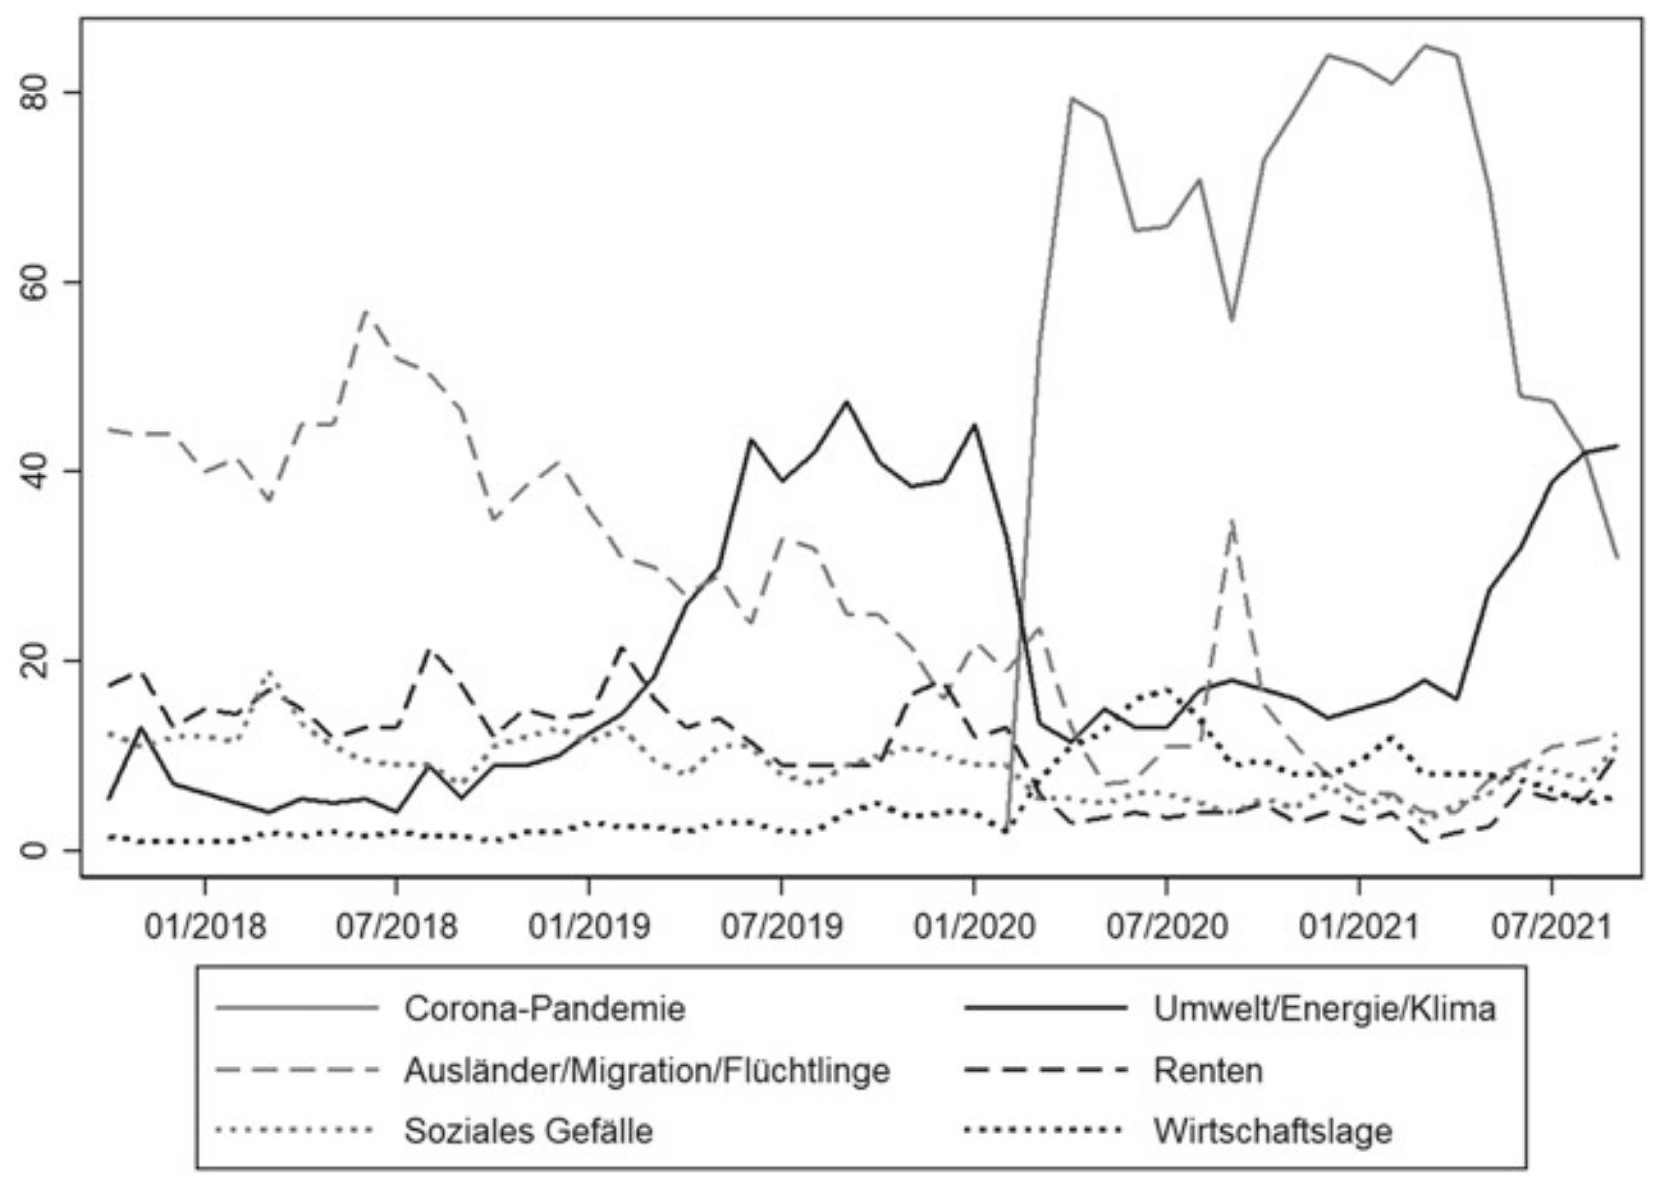
\includegraphics[width=0.8\textwidth]{data/images/themenkonjunktur.png}
  \caption{Verlauf der wichtigsten politischen Themen während der 19. Wahlperiode \autocite{engler_wettbewerb_2022, forschungsgruppe_wahlen_forschungsgruppe_nodate}} \label{fig:themenkonjunktur}
\end{figure}

Zu Beginn der Legislaturperiode war das Thema der Migrationspolitik am wichtigsten. Die Relevanz hat jedoch stetig abgenommen, bis das Thema ab \num{2020} untergeordnet war. Der Themenbereich Umwelt, Energie und Klima wurde ab \num{2019} immer wichtiger und war zeitweise das Thema mit der meisten Relevanz. Nach der Flutkatastrophe \num{2021} wurde diesem Bereich erneut vermehrt Bedeutung zugesprochen. Nach dem Ausbruch der Pandemie war diese schlagartig das mit Abstand dominierende Thema, bis sich die Lage ab \num{2021} wieder beruhigte. Während des gesamten Zeitraums rückten wirtschafts- und sozialpolitische Themen in den Hintergrund.

Gemäß \textcite{niedermayer_entwicklung_2020} waren im Betrachtungszeitraum vor allem die Flüchtlingskrise sowie das Thema Klimawandel und Energiewende von Bedeutung. Die Dominanz der Klimathematik zeigt sich an Ereignissen wie dem Dieselskandal, der Hitzewelle im Sommer \num{2018} sowie der Popularität der Protestbewegung \enquote{Fridays for Future}.

\section{Repräsentationsformen von Text} \label{sec:representationForms}

Um Analysen und \ac{ML} auf Texten anwenden zu können, ist es notwendig, diese in Vektoren umzuwandeln, die von Maschinen interpretiert werden können. Dafür existieren unterschiedliche Verfahren, die unter anderem den Kontext und komplexe semantische Beziehungen berücksichtigen \autocite{kowsari_text_2019, jurafsky_speech_2023}.

Kontextunabhängige Methoden wie \ac{BoW} und \ac{TF-IDF} extrahieren Informationen über die Häufigkeit einzelner Wörter. \ac{GloVe} stellt eine komprimierte Worteinbettungsmethode dar, die auf der Basis von Kookkurrenzstatistiken und der Verteilung der Wörter im Korpus beruht. Mit diesen Verfahren kann meist nur die Semantik eines Satzes rudimentär abgebildet werden, da jegliche Informationen über den aktuellen Kontext fehlen. Ein alternativer Ansatz ist die Repräsentation mittels kontextabhängigen Verfahren. Neuronale Netze, unter anderem \ac{LSTM}-Netzwerke und Transformer-basierte Modelle, sind in der Lage, Zusammenhänge innerhalb eines Satzes zu erkennen. \ft berücksichtigt Subwort-Informationen, weshalb es kontextabhängig ist. Zudem ermöglicht es, einfache semantische Zusammenhänge abzubilden.

Worteinbettungen (engl. Word Embeddings) spielen eine zentrale Rolle bei der Analyse und dem Training von \ac{NLP}-Modellen. Diese stellen einzigartige Wörter mittels mehrdimensionalen Vektoren\footnote{Häufig bestehen Word Embeddings aus \num{300} Dimensionen} dar. Je nach Verfahren können die resultierenden Vektoren komprimiert oder unkomprimiert sein. Worteinbettungen ermöglichen es, Wörter mit ähnlicher Bedeutung im mehrdimensionalen Raum zu gruppieren.

Die unterschiedlichen Verfahren können auf Wort-, Satz- oder Dokumentebene angewendet werden.

\subsection*{N-Gram}

N-Grams bilden die Grundlage für Verfahren wie \ac{BoW} und \ft. Bei dieser Methode werden Zeichen (auf Wortebene) oder Wörter (auf Satzebene) in Fragmente der Länge \texttt{n} unterteilt \autocite[5]{kowsari_text_2019}. Die Reihenfolge der Elemente bleibt dabei unverändert.

\subsection*{\acl{BoW}}

\ac{BoW} ist eine einfache Repräsentationsform, die lediglich die Häufigkeit von einzigartigen Wörtern berechnet \autocite[6]{kowsari_text_2019}. Im ersten Schritt des Verfahrens wird ein Satz oder Dokument in eine Menge an 1-Grams (einzelne Wörter) transformiert. Anschließend wird die Liste auf die einzigartigen Wörter reduziert und gezählt, wie häufig die einzigartigen Wörter (engl. Features) auftreten. Die daraus resultierende Tabelle wird auch \ac{BoF} genannt.

Um zu demonstrieren, wie \ac{BoW} funktioniert, nennt \textcite[6]{kowsari_text_2019} folgendes Beispiel: \enquote{As the home to UVA’s recognized undergraduate and graduate degree programs in systems engineering. In the UVA Department of Systems and Information Engineering, our students are exposed to a wide range of range.} Aus dem Text resultiert die folgende \ac{BoF}-Tabelle: \enquote{\{1,1,1,3,2,1,2,1,2,3,1,1,1,2,1,1,1,1,1,1\}}.

Aufgrund des fehlenden syntaktischen Verständnisses kann \ac{BoW} zum Beispiel nicht zwischen \textit{\enquote{Das ist gut}} und \textit{\enquote{Ist das gut}} unterscheiden \autocite[6]{kowsari_text_2019}.

\subsection*{\acl{TF-IDF}}

Neben der reinen Häufigkeit berücksichtigt \ac{TF-IDF} auch die Häufigkeit eines Wortes innerhalb einer Sammlung von Dokumenten \autocite[7]{kowsari_text_2019}. Damit ist es möglich, Wörter aus Wortgruppen wie Artikeln, Präpositionen und Konjunktionen von relevanten Wörtern (meist Adjektive, Verben und Nomen) zu trennen.

\[\mathrm{tfidf}(t,d,D) = \frac{f_{t,d}}{{\sum_{t' \in d}{f_{t',d}}}} \cdot \log \frac{N}{|\{d \in D: t \in d\}|}\]

Zunächst wird die relative oder absolute Häufigkeit eines Wortes innerhalb eines Dokuments berechnet. Zudem wird die Häufigkeit in anderen Dokumenten ermittelt. Der sich daraus ergebende Wert gibt Auskunft darüber, ob es sich um ein generell häufiges Wort handelt oder nicht.

\subsection*{GloVe}

\ac{GloVe} repräsentiert jedes Wort als hochdimensionalen Vektor \autocite[8\psq]{kowsari_text_2019}. Aufgrund der umfangreichen Datenmengen, die für das Training benötigt werden, ist es üblich, vortrainierte Wortvektoren zu verwenden. \citeauthor{kowsari_text_2019} gibt an, dass hierfür Datensätze wie Wikipedia und Gigaword \num{5} verwendet werden. Die erzeugten Wortvektoren sind dann in der Lage, sprachliche oder semantische Ähnlichkeiten mittels der Euklidischen Distanz festzustellen \autocite{pennington_glove_2014}. Zusätzlich weisen die Wortvektoren lineare Unterstrukturen auf.

\begin{figure}[H]
  \centering
  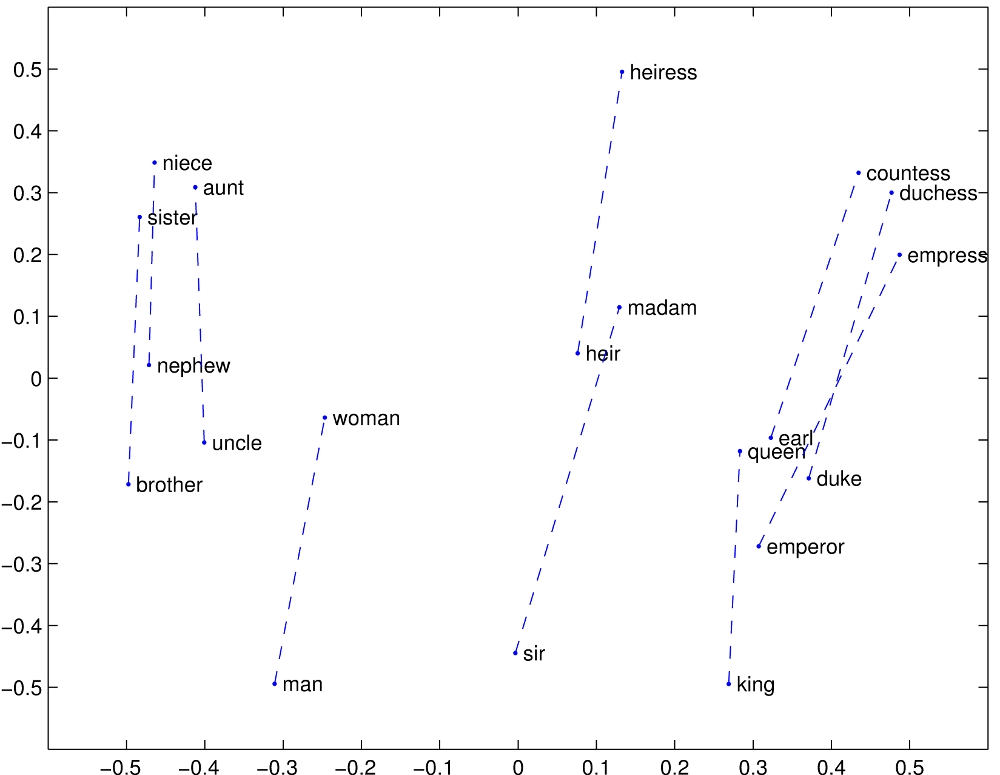
\includegraphics[width=0.6\textwidth]{data/images/materials_and_methods/man_woman.jpg}
  \caption{Beispiel \autocite{Mann - Frau} mittels \acs{GloVe} \autocite{pennington_glove_2014}} \label{fig:gloveExample}
\end{figure}

Das in \autoref{fig:gloveExample} gezeigte Beispiel ist eine der am häufigsten verwendeten Veranschaulichungen von \ac{GloVe}. Die Grafik zeigt diverse Wörter in einem zweidimensionalen Raum. Aufgrund der linearen Unterstrukturen lassen sich Wörter addieren und subtrahieren. So ergibt beispielsweise \(king - man + woman = queen\). Es ist jedoch zu beachten, dass \ac{GloVe} ausschließlich mit Wörtern funktioniert, auf denen es auch trainiert wurde.

\subsection*{Embedding-Schicht in neuronalen Netzwerken}

Um Worteinbettungen in neuronalen Netzwerken zu nutzen, wird eine Embedding-Schicht benötigt, die den Eingabetext in eine Sequenz von Wortvektoren umwandelt. Diesen Prozess stellt \autoref{fig:embeddingLayer} dar.

\begin{figure}[H]
  \centering
  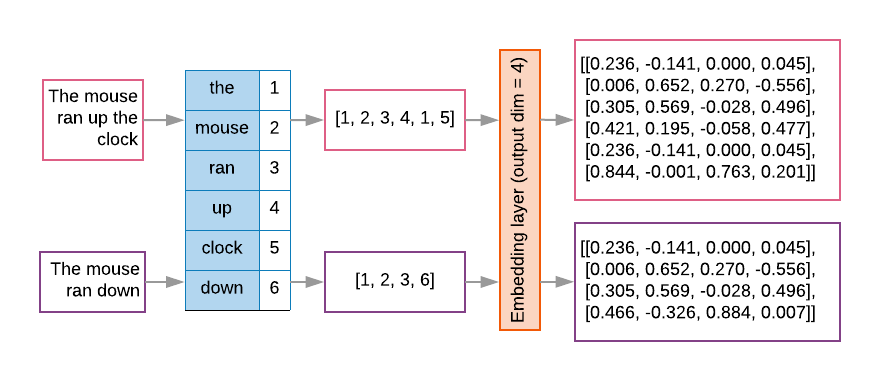
\includegraphics[width=0.8\textwidth]{data/images/embedding_layer.png}
  \caption{Funktionsweise der Embedding-Schicht \autocite{google_prepare_2022}} \label{fig:embeddingLayer}
\end{figure}

Zunächst muss ein Wort-Index basierend auf allen Trainingstexten erstellt werden, der jedem im Datensatz vorkommenden Wort einen eindeutigen Index zuweist. Mit diesem kann jeder Text in eine Abfolge von Indizes umgewandelt werden. In der Embedding-Schicht wird jeder dieser Indizes durch den Vektor ersetzt, der das entsprechende Wort repräsentiert. Die Länge des Vektors ist abhängig von den Dimensionen, die die Worteinbettungen bereitstellen. Als Endergebnis entsteht pro Text eine Liste aus Wortvektoren für jedes Wort im Eingabetext, die an die weiteren Schichten des Netzes weitergegeben wird.

\subsection*{fastText}

Anstelle von ganzen Wörtern verwendet \ft zum Trainieren und Klassifizieren n-grams, die aus \textit{n} Zeichen bestehen \autocite{kowsari_text_2019, joulin_fasttextzip_2016}. Ein Beispiel ist das Wort \textit{Tischtennis}, das mit \(n = 3\) in \textit{<Ti,Tis,isc,sch,cht,hte,ten,enn,nni,nis,is>} zerlegt wird. Wörter, die in ähnliche n-grams zerlegt werden können, resultieren in Vektoren, die nah im Vektorraum liegen. Die Optimierung während des Trainings und der Klassifikation erfolgt mittels der Softmax-Funktion. Zusätzlich wird bag-of-n-grams genutzt, um Zusammenhänge in einem Text zu erkennen \autocite[2]{joulin_bag_2016}. Aufgrund der n-gram Methodik und der niedrigen Komplexität von \(O(h \log_{2}(k))\) des Optimierungs- und Klassifikationsverfahrens, eignet sich \ft für die Klassifikation von großen Mengen an Text \autocite[2\psqq]{joulin_bag_2016}.

Im Vergleich zu \ac{GloVe} lassen sich mit \ft auch Wörter klassifizieren, die im Datensatz enthalten sind \autocite{guhr_training_2020, bojanowski_enriching_2017}. Das ist besonders bei komplexen Sprachen wie Deutsch hilfreich, die zusammengesetzte Wörter verwenden. Ein Beispiel ist das Wort Tischtennis, das im Englischen \textit{table tennis} lautet.

\subsection*{BERT}

Bei \ac{BERT} handelt es sich um ein tiefes neuronales Netz. Das Modell beruht auf der Transformer-Architektur \autocite[3]{devlin_bert_2019}. Durch den bidirektionalen Ansatz ist es möglich, den Kontext eines Satzes deutlich besser zu verstehen. Das liegt daran, dass vorherige Modelle ausschließlich von vorne nach hinten oder umgekehrt einen Satz verarbeiten konnten. \ac{BERT} hingegen verarbeitet den gesamten Satz gleichzeitig. Im Trainingsprozess werden zufällig Wörter maskiert \autocite[4]{devlin_bert_2019}. Die Autoren beschreiben außerdem, dass das Modell den nachfolgenden Satz vorhersagt und abgleicht. Beide Methoden helfen dabei, gezielt Eigenschaften der Trainingsdaten zu erlernen.

Neben englischsprachigen Modellen finden sich ebenfalls deutsche. Weiterhin existieren reduzierte Modelle, wie DistilBERT, die weniger Ressourcen benötigen, ohne größere Performance-Einbußen zu verzeichnen.

\section{Sentimentanalyse} \label{sec:sentimentanalysis}

Herkömmliche Methoden zur Bestimmung des Sentiments von deutschen Texten sind Sentiment-Wörterbücher und \ac{ML}-Modelle wie \ac{SVM}, \ac{CNN} und \ac{LSTM} \autocite[1627\psq]{guhr_training_2020}. Alle genannten Methoden erreichen einen $F_1$ Score zwischen \numrange{46.5}{74.9}.

Die Arbeit von \textcite{guhr_training_2020} zeigt auf, wie Texte anhand ihres Sentiments -- positiv, neutral oder negativ -- mithilfe von \ac{BERT} klassifiziert werden können. Für das Training verwendeten die Autoren acht unterschiedliche Datensätze, die insgesamt \num{5.3} Millionen Einträge umfassen. Neben einem \ac{BERT}-Modell wurde auch ein Modell mittels \ft trainiert. Dieses erzielt jedoch einen leicht schlechteren $F_1$ Score\footnote{Mit dem unausgeglichenen Datensatz erzielt \ac{BERT} einen $F_1$ Score von \num{97.44} und \ft \num{95.73}. Mit dem ausgeglichenen Datensatz erreicht \ac{BERT} einen $F_1$ Score von \num{96.36} und \ft \num{94.05}.} als das \ac{BERT}-Modell \autocite[\psq 1630]{guhr_training_2020}.

Auffällig ist, dass das Modell einen signifikant schlechteren $F_1$ Score erzielt, wenn der Datensatz Tweets oder andere Social Media Beiträge einschließt. Dies zeigt sich bei den Datensätzen PlotTS, SB10k und GermEval-2017. Bei der Klassifikation dieser erreicht das Modell lediglich einen $F_1$ Score zwischen \numrange{0.6423}{0.7885} \autocite[1631]{guhr_training_2020}.

\section{Zusammenfassung}

Der erste Abschnitt dieses Kapitels skizziert die politische Situation in Deutschland während der \num{19}. Legislaturperiode. Die Volksparteien \ac{CDU}/\ac{CSU} und \ac{SPD} mussten bei der Bundestagswahl \num{2017} Verluste hinnehmen, bilden jedoch eine Große Koalition. Die Grünen und die \ac{AfD} verzeichneten einen Aufschwung, was zu einer Diversifizierung des Parteiensystems führte. Im Untersuchungszeitraum dominierten hauptsächlich die Themenbereiche Migration, Klimaschutz und Pandemie den Diskurs.

Der zweite Abschnitt des Kapitels umreißt die Grundmethoden zur Analyse und Klassifizierung von Texten. \ac{BoW} und \ac{TF-IDF} sind die beiden grundlegenden Methoden, die lediglich die Häufigkeit einzigartiger Wörter berücksichtigen. \ac{BoW} betrachtet dabei ein einzelnes Dokument, während \ac{TF-IDF} auch die Häufigkeit über mehrere Dokumente hinweg berücksichtigt. Im Gegensatz zu diesen beiden unkomprimierten Verfahren verwenden Word2Vec, GloVe und \ft komprimierte Vektoren, die Wörter oder Zeichen basierend auf ihrem Kontext einem Vektor im Vektorraum zuordnen.

Für die Analyse mittels deskriptiver Statistik in \autoref{ch:crispDm_1} wird ein Modell zur Bestimmung der Stimmung eines Textes betrachtet. Dieses Modell gibt Aufschluss darüber, ob ein Text positiv, negativ oder neutral klingt.
